\documentclass{article}
\usepackage[utf8]{inputenc}
\usepackage{graphicx}

\title{Advanced ZombieRun}     %% \title est une macro, entre { } figure son premier argument
\author{Tom BESSON\\ Willy FRANÇOIS\\ Jean-Baptiste PERRIN\\ Joris RUBAGOTTI}
\makeindex

\begin{document}


\maketitle


\newpage


\tableofcontents


\newpage


\section{Introduction}


Pour la réalisation d'un projet dans le cadre de la matière de développement d'application nomade, nous avons décidé de créer un jeu intitulé Advanced\\ ZombieRun.

Le jeu consiste en la réalisation d'un parcourt d'un point de départ vers un point d'arrivée choisit par le joueur sur une map avec pour détermination de la position de celui-ci l'utilisation du GPS. Mais le jeu génère aléatoirement des Zombies virtuels ayant pour but d'intercepter le joueur et ainsi l'empêcher de gagner la partie.
La condition de victoire est d'arriver sur le point d'arrivée sans avoir été touché par les zombies.

Nous vous présenterons tout au long du rapport les différentes phases du développement, les problèmes rencontrés et les améliorations possibles dans l'avenir.


\section{Les choix de développement}

Pour le développement du projet, notre groupe a fait le choix de permettre à la majorité des appareils mobiles tournant sous les différentes version d'Android puissent accueillir l'application. Pour ce faire, nous avons développé l'application pour qu'elle fonctionne pour les versions d'Android de la 2.2 à la 4.2(La plus récente au moment ou nous écrivons ces mots) mais cela nous a apporté quelques contraintes sur l'utilisation de certaines fonctionnalités de l'API d'Android. Par exemple, l'utilisation du Wifi Direct nous était impossible car celui-ci n'est supporté qu'à partir de la version 4.0.3 d'Android et la majorité des portables aujourd'hui n'en sont toujours pas équipé.
Pour l'affichage de la map lors du jeu, nous avons choisit d'utiliser l'API GoogleMap.  

\newpage

\section{La structure du projet}


\subsection{HomeActivity}

Cette activité représente le menu principal de notre projet avec le choix d'une partie solo ou multijoueur.


\vfill
\begin{center} 
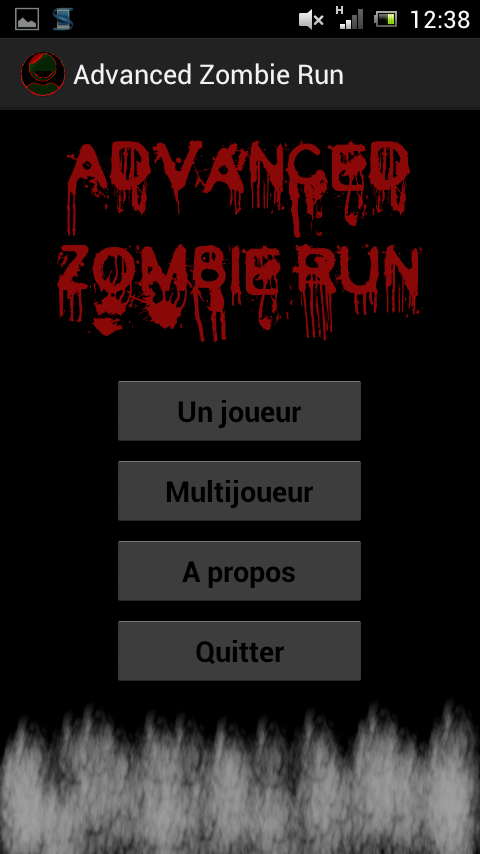
\includegraphics[width=4.2cm, height=7.cm]{menu.png}
\end{center}
\vfill


\subsection{PreferencesActivity}


Cette activité permet de définir les différents paramètres de la partie. On peut y choisir:
\begin{itemize}
\item Notre nom pour les parties multijoueurs
\item La densité de la population de zombies
\item Leur vitesse de déplacement
\item Le temps imparti pour arriver à destination
\item Notre nombre de points de vie
\item Le type d'alerte en cas de contact
\end{itemize}
Les choix faits par l'utilisateur sont enregistrés dans les SharedPreferences du projet afin d'être récupérés plus tard dans la Map.


\subsection{Map}

Afin de pouvoir afficher une carte, nous avons dû utiliser l'API Google Maps. Cette API permet d'afficher une carte dans Android avec le widget \emph{MapView} et une activité héritant de \emph{MapActivity}. Cette API permet de manipuler cette \emph{MapView}, dans le but d'afficher ou manipuler des marqueurs, calculer des distances entre 2 points géographiques.   

\vfill
\begin{center} 
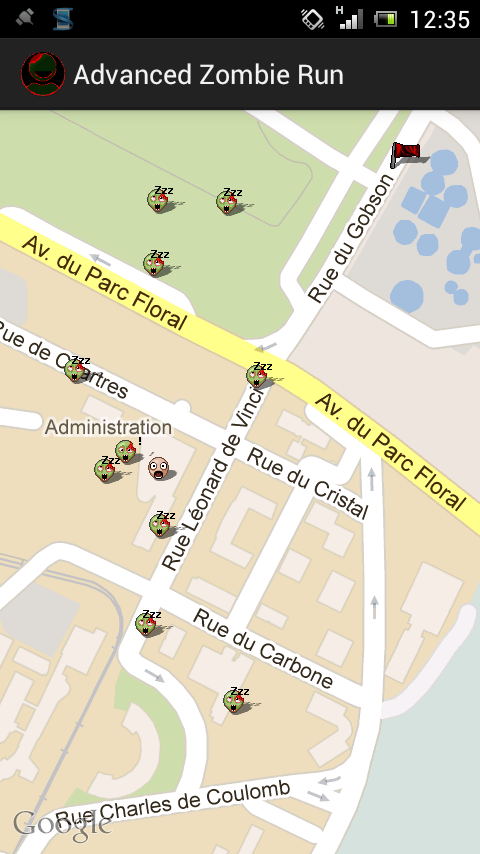
\includegraphics[width=4.2cm, height=7.cm]{game.png}
\end{center}
\vfill

\subsection{GameMaster}

Le GameMaster permet la gestion du jeu en lui-même. C'est lui qui va calculer tout d'abord l'emplacement d'apparition des zombies sur la carte et par la suite leurs déplacements. Ces calculs exploitent des principes mathématiques propre au fonctionnement d'un GPS. Tout cela est utilisé par la Map, qui va transférer au GameMaster les nouvelles coordonnées des joueurs, dont il va se servir pour trouver les nouvelles coordonnées des zombies.

\subsection{GameEndActivity}

Cette activité s'affiche lorsque le jeu touche à sa fin. Si vous êtes mort au cours du jeu, la page indiquera votre mort, si vous avez gagner en arrivant au point d'arrivé, la l'activité indiquera la victoire.

\subsection{AboutActivity}

Cette activité contient le noms des participants à la réalisation du projet.

\subsection{MultiplayerActivity}

Cette activité accueil le joueur si il a fait le choix du multijoueur. Quand le joueur arrive dessus, celui-ci doit activer son bluetooth pour le multijoueur. Elle permet de créer une partie en tant qu'hébergeur de celle-ci renvoyant ainsi vers PreferenceActivity. Sinon il y a aussi la possibilité d'en rejoindre une via la listview affichant les partie disponibles (hélas fonctionnalité non mise en place dû à un problème rencontré lors du développement).  

\subsection{RoomStayHostActivity}

Après que l'hébergeur ait choisit les préférences de partie ou que le client ait fait le choix de rejoindre une partie, il arrive sur cette activité. Mais suite aux différents problèmes de développements sur le multijoueur, cette activité n'offre pas la possibilité de continuer plus loin. 

\section{Les problèmes rencontrés}

\subsection{Problème de détermination de position}

Au cours du développement de l'application, nous avons étés confrontés à plusieurs problèmes. Le plus gênant de ces problèmes est celui du déplacement des zombies qui ne se faisait pas comme il fallait.
Les différents calculs afin de trouver la position future d'un zombie en fonction de sa position actuelle, son angle de direction, et sa distance parcourue nous ont donnés du fil à retordre étaient notre première approche, mais nous avons ensuite opté par un calcul bien plus simple utilisant le théorème de Thalès.


\subsection{Problème multijoueur}

Le multijoueur a aussi posé quelques soucis. 
Initialement, le multijoueur devait permettre à plusieurs joueurs de jouer ensemble sur une même partie via le Wi-Fi ou le BlueTooth. Après que les joueurs se soit rejoint, l'hôte envoyait aux différents clients la position du point d'arrivée puis la positions des zombies sur la Map. Ensuite le portable du client devait envoyé sa nouvelle position à l'hôte. De cette manière chaque joueur possédait un détecteur sur son portable et une map à lui.    
Dans un premier temps nous étions partit sur l'idée d'utiliser le hotspot du Wi-Fi pour les transactions ce qui nous semblait être une bonne idée de par sa capacité à permettre l'échange de données entre les différents appareils qui y sont reliés et sa portée,
mais l'hébergeur l'utilisant n'avait aucun accès aux clients qui se connectaient à lui.
Nous sommes donc partis sur le BlueTooth, en détresse, vers la fin du projet mais faute de temps le multijoueur n'a pas pu être mis en place.

\newpage

\section{Les améliorations possibles dans l'avenir}


Dans l'avenir, nous pourrions rendre fonctionnel le multijoueur afin d'offrir une expérience inédite aux utilisateurs de l'application. D'autres ajouts sont possibles comme des modes de jeux dérivés de l'original offrant ainsi plus de variétés pour celui-ci. 


\section{Conclusion}

On peut conclure que l'on a peut être sous estimé l'importance du projet en lui-même. Le développement s'est retrouvé bien plus compliqué que prévu et le manque d'informations sur certaines fonctionnalités d'un mobile Android (exemple : le hotspot) nous a fait perdre du temps sur le développement. Mais ce projet s'est révélé tout de même intéressant en nous apportant plus de connaissance sur le système Android.

Mais au final, nous avons une application qui fonctionne en "Un Joueur".
Nous pouvons placer une destination. Ensuite, des zombis apparaissent et se déplacent aléatoirement.
Une fois qu'un zombi nous a repéré, il nous prend en chasse.
Et si l'un d'eux est trop loin des joueurs, il est supprimé et un nouveau sera créé dans la zone autour des joueurs.
  

\end{document} 